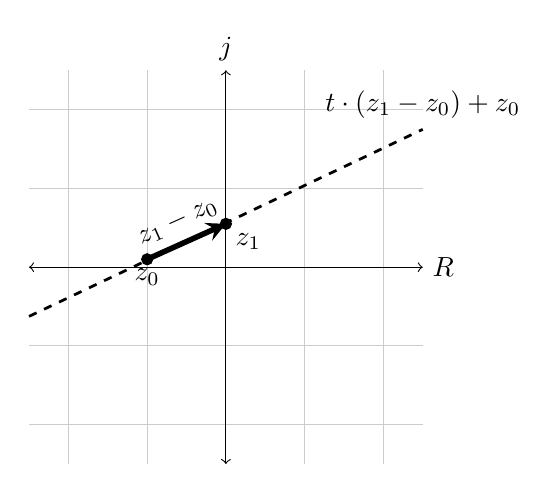
\begin{tikzpicture}
    \draw [thin,gray!40] (-2.5,-2.5) grid (2.5,2.5);
    \draw[<->] (-2.5,0)--(2.5,0) node[right] {$R$};
    \draw[<->] (0,-2.5)--(0,2.5) node[above]{$j$};
    \coordinate (a) at (-1,0.1);
    \coordinate (b) at (-0,0.55);
    \draw[fill=black] (a) circle(2pt) node[below]{$z_0$};
    \draw[fill=black] (b) circle(2pt) node[anchor=north west]{$z_1$};
    \draw[line width=2pt,black,-stealth] (a)--(b) node[midway, above, sloped]{$z_1-z_0$};
    \draw[line width=1pt,black,dashed] (-2.5,-0.625)--(2.5,1.75) node[above]{$t\cdot(z_1-z_0)+z_0$};
\end{tikzpicture}
\caption*{Ecuación de la recta desplazada}